
\section{Wind rose}

A wind rose is a graphic tool used by meteorologists to give a succinct view of how wind speed and direction are typically distributed at a particular location. Historically, wind roses were predecessors of the compass rose, as there was no differentiation between a cardinal direction and the wind which blew from such a direction. Using a polar coordinate system of gridding, the frequency of winds over a time period is plotted by wind direction, with color bands showing wind speed ranges. The direction of the longest spoke shows the wind direction with the greatest frequency(\cite{wikipedia}). \par

% \textcite{parish2009propagation}

\section{Data source}
The wind data is obtained directly from the SmartAtlantic Alliance which is an initiative of the Fisheries and Marine Institute of Memorial University of Newfoundland's Centre for Applied Ocean Technology (CTec) and the Centre for Ocean Ventures and Entrepreneurship (COVE) of Halifax.\par
The URL of CSV data file can be generated from their website as the figure shown below.\par

\begin{figure}[h!]
    \centering
    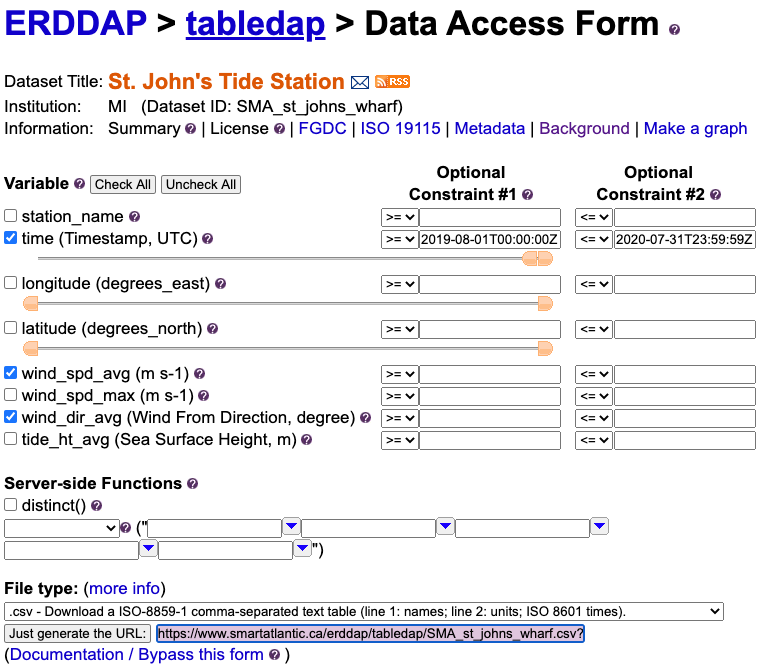
\includegraphics[width=0.50\textwidth]{images/data_source.png}
    \caption{URL generation of CSV data file}
    \label{fig: PaleBlueDot}    
\end{figure}

In this project, the information of timestamp, wind speed and wind direction in the last 365 days (from 1 August 2019 to 31 July 2020) was collected and used to plot wind rose.\par

\section{Analysis workflow}
